%        File: arfc-beamer.tex
%     Created: Sun May 5 10:00 PM 2013 C


%\documentclass[11pt,handout]{beamer}
\documentclass[9pt]{beamer}
\usetheme[white]{Illinois}
%\title[short title]{long title}
\title[Safety analysis]{Safety Analysis of the Molten Salt Fast Reactor Fuel
Composition with Moltres}
%\subtitle[short subtitle]{long subtitle}
%\subtitle[Brief Summary]{A Brief Summary}
%\author[short name]{long name}
\author[Authors]{Sun Myung Park$^1$, Andrei Rykhlevskii$^1$, and Kathryn D.
Huff$^1$}
%\date[short date]{long date}
\date[09.24.2019]{September 24, 2019}
%\institution[short name]{long name}
\institute{
$^1$Dept. of Nuclear, Plasma and Radiological Engineering, University of
Illinois at Urbana-Champaign \\
}

%\usepackage{bbding}
\usepackage{amsfonts}
\usepackage{amsmath}
\usepackage{xspace}
\usepackage{graphicx}
\usepackage{subfigure}
\usepackage{booktabs} % nice rules for tables
\usepackage{microtype} % if using PDF
\usepackage{bigints}
\usepackage{minted}
\usepackage[absolute,overlay]{textpos}
\usepackage{tikz}
\usetikzlibrary{positioning, arrows, decorations, shapes}
\usetikzlibrary{shapes.geometric,arrows}
\definecolor{illiniblue}{HTML}{B1C6E2}
\tikzstyle{bblock} = [rectangle, draw, fill=illiniblue, 
text width=10em, text centered, rounded corners, minimum height=4em]
\tikzstyle{sbblock} = [rectangle, draw, fill=illiniblue, 
text width=7em, text centered, rounded corners, minimum height=4em]
\tikzstyle{arrow} = [thick,->,>=stealth]

\newcommand{\units}[1] {\:\text{#1}}%
\newcommand{\SN}{S$_N$}%{S$_\text{N}$}%{$S_N$}%
\DeclareMathOperator{\erf}{erf}
%I need some complimentary error funcitons... 
\DeclareMathOperator{\erfc}{erfc}
%Those icons in the references are terrible looking
\setbeamertemplate{bibliography item}[text]

%%%% Acronym support

\usepackage[acronym,toc]{glossaries}
%\newacronym{<++>}{<++>}{<++>}
\newacronym[longplural={metric tons of heavy metal}]{MTHM}{MTHM}{metric ton of heavy metal}
\newacronym{ABM}{ABM}{agent-based modeling}
\newacronym{ACDIS}{ACDIS}{Program in Arms Control \& Domestic and International Security}
\newacronym{AHTR}{AHTR}{Advanced High Temperature Reactor}
\newacronym{ANDRA}{ANDRA}{Agence Nationale pour la gestion des D\'echets RAdioactifs, the French National Agency for Radioactive Waste Management}
\newacronym{ANL}{ANL}{Argonne National Laboratory}
\newacronym{API}{API}{application programming interface}
\newacronym{ARE}{ARE}{Aircraft Reactor Experiment}
\newacronym{ARFC}{ARFC}{Advanced Reactors and Fuel Cycles}
\newacronym{ASME}{ASME}{American Society of Mechanical Engineers}
\newacronym{ATWS}{ATWS}{Anticipated Transient Without Scram}
\newacronym{BDBE}{BDBE}{Beyond Design Basis Event}
\newacronym{BIDS}{BIDS}{Berkeley Institute for Data Science}
\newacronym{BOL}{BOL}{beginning of life}
\newacronym{CAFCA}{CAFCA}{ Code for Advanced Fuel Cycles Assessment }
\newacronym{CDTN}{CDTN}{Centro de Desenvolvimento da Tecnologia Nuclear}
\newacronym{CEA}{CEA}{Commissariat \`a l'\'Energie Atomique et aux \'Energies Alternatives}
\newacronym{CI}{CI}{continuous integration}
\newacronym{CNEN}{CNEN}{Comiss\~{a}o Nacional de Energia Nuclear}
\newacronym{CNERG}{CNERG}{Computational Nuclear Engineering Research Group}
\newacronym{COSI}{COSI}{Commelini-Sicard}
\newacronym{COTS}{COTS}{commercial, off-the-shelf}
\newacronym{CSNF}{CSNF}{commercial spent nuclear fuel}
\newacronym{CTAH}{CTAHs}{Coiled Tube Air Heaters}
\newacronym{CUBIT}{CUBIT}{CUBIT Geometry and Mesh Generation Toolkit}
\newacronym{CURIE}{CURIE}{Centralized Used Fuel Resource for Information Exchange}
\newacronym{DAG}{DAG}{directed acyclic graph}
\newacronym{DANESS}{DANESS}{Dynamic Analysis of Nuclear Energy System Strategies}
\newacronym{DBE}{DBE}{Design Basis Event}
\newacronym{DESAE}{DESAE}{Dynamic Analysis of Nuclear Energy Systems Strategies}
\newacronym{DHS}{DHS}{Department of Homeland Security}
\newacronym{DOE}{DOE}{Department of Energy}
\newacronym{DRACS}{DRACS}{Direct Reactor Auxiliary Cooling System}
\newacronym{DRE}{DRE}{dynamic resource exchange}
\newacronym{DSNF}{DSNF}{DOE spent nuclear fuel}
\newacronym{DYMOND}{DYMOND}{Dynamic Model of Nuclear Development }
\newacronym{EBS}{EBS}{Engineered Barrier System}
\newacronym{EDZ}{EDZ}{Excavation Disturbed Zone}
\newacronym{EIA}{EIA}{U.S. Energy Information Administration}
\newacronym{EOL}{EOL}{end of life}
\newacronym{EPA}{EPA}{Environmental Protection Agency}
\newacronym{EP}{EP}{Engineering Physics}
\newacronym{FCO}{FCO}{Fuel Cycle Options}
\newacronym{FCT}{FCT}{Fuel Cycle Technology}
\newacronym{FEHM}{FEHM}{Finite Element Heat and Mass Transfer}
\newacronym{FEPs}{FEPs}{Features, Events, and Processes}
\newacronym{FHR}{FHR}{Fluoride-Salt-Cooled High-Temperature Reactor}
\newacronym{FLiBe}{FLiBe}{Fluoride-Lithium-Beryllium}
\newacronym{GDSE}{GDSE}{Generic Disposal System Environment}
\newacronym{GDSM}{GDSM}{Generic Disposal System Model}
\newacronym{GENIUSv1}{GENIUSv1}{Global Evaluation of Nuclear Infrastructure Utilization Scenarios, Version 1}
\newacronym{GENIUSv2}{GENIUSv2}{Global Evaluation of Nuclear Infrastructure Utilization Scenarios, Version 2}
\newacronym{GENIUS}{GENIUS}{Global Evaluation of Nuclear Infrastructure Utilization Scenarios}
\newacronym{GPAM}{GPAM}{Generic Performance Assessment Model}
\newacronym{GRSAC}{GRSAC}{Graphite Reactor Severe Accident Code}
\newacronym{GUI}{GUI}{graphical user interface}
\newacronym{HLW}{HLW}{high level waste}
\newacronym{HPC}{HPC}{high-performance computing}
\newacronym{HTC}{HTC}{high-throughput computing}
\newacronym{HTGR}{HTGR}{High Temperature Gas-Cooled Reactor}
\newacronym{IAEA}{IAEA}{International Atomic Energy Agency}
\newacronym{IEMA}{IEMA}{Illinois Emergency Mangament Agency}
\newacronym{INL}{INL}{Idaho National Laboratory}
\newacronym{IPRR1}{IRP-R1}{Instituto de Pesquisas Radioativas Reator 1}
\newacronym{IRP}{IRP}{Integrated Research Project}
\newacronym{ISFSI}{ISFSI}{Independent Spent Fuel Storage Installation}
\newacronym{ISRG}{ISRG}{Independent Student Research Group}
\newacronym{JFNK}{JFNK}{Jacobian-Free Newton Krylov}
\newacronym{LANL}{LANL}{Los Alamos National Laboratory}
\newacronym{LBNL}{LBNL}{Lawrence Berkeley National Laboratory}
\newacronym{LCOE}{LCOE}{levelized cost of electricity}
\newacronym{LDRD}{LDRD}{laboratory directed research and development}
\newacronym{LFR}{LFR}{Lead-Cooled Fast Reactor}
\newacronym{LLNL}{LLNL}{Lawrence Livermore National Laboratory}
\newacronym{LMFBR}{LMFBR}{Liquid Metal Fast Breeder Reactor}
\newacronym{LOFC}{LOFC}{Loss of Forced Cooling}
\newacronym{LOHS}{LOHS}{Loss of Heat Sink}
\newacronym{LOLA}{LOLA}{Loss of Large Area}
\newacronym{LP}{LP}{linear program}
\newacronym{LWR}{LWR}{Light Water Reactor}
\newacronym{MA}{MA}{minor actinide}
\newacronym{MCNP}{MCNP}{Monte Carlo N-Particle code}
\newacronym{MILP}{MILP}{mixed-integer linear program}
\newacronym{MIT}{MIT}{the Massachusetts Institute of Technology}
\newacronym{MOAB}{MOAB}{Mesh-Oriented datABase}
\newacronym{MOOSE}{MOOSE}{Multiphysics Object-Oriented Simulation Environment}
\newacronym{MOX}{MOX}{mixed oxide}
\newacronym{MSBR}{MSBR}{Molten Salt Breeder Reactor}
\newacronym{MSFR}{MSFR}{Molten Salt Fast Reactor}
\newacronym{MSRE}{MSRE}{Molten Salt Reactor Experiment}
\newacronym{MSR}{MSR}{Molten Salt Reactor}
\newacronym{NAGRA}{NAGRA}{National Cooperative for the Disposal of Radioactive Waste}
\newacronym{NEAMS}{NEAMS}{Nuclear Engineering Advanced Modeling and Simulation}
\newacronym{NEUP}{NEUP}{Nuclear Energy University Programs}
\newacronym{NFCSim}{NFCSim}{Nuclear Fuel Cycle Simulator}
\newacronym{NGNP}{NGNP}{Next Generation Nuclear Plant}
\newacronym{NMWPC}{NMWPC}{Nuclear MW Per Capita}
\newacronym{NNSA}{NNSA}{National Nuclear Security Administration}
\newacronym{NPRE}{NPRE}{Department of Nuclear, Plasma, and Radiological Engineering}
\newacronym{NQA1}{NQA-1}{Nuclear Quality Assurance - 1}
\newacronym{NRC}{NRC}{Nuclear Regulatory Commission}
\newacronym{NSF}{NSF}{National Science Foundation}
\newacronym{NSSC}{NSSC}{Nuclear Science and Security Consortium}
\newacronym{NUWASTE}{NUWASTE}{Nuclear Waste Assessment System for Technical Evaluation}
\newacronym{NWF}{NWF}{Nuclear Waste Fund}
\newacronym{NWTRB}{NWTRB}{Nuclear Waste Technical Review Board}
\newacronym{OCRWM}{OCRWM}{Office of Civilian Radioactive Waste Management}
\newacronym{ORION}{ORION}{ORION}
\newacronym{ORNL}{ORNL}{Oak Ridge National Laboratory}
\newacronym{PARCS}{PARCS}{Purdue Advanced Reactor Core Simulator}
\newacronym{PBAHTR}{PB-AHTR}{Pebble Bed Advanced High Temperature Reactor}
\newacronym{PBFHR}{PB-FHR}{Pebble-Bed Fluoride-Salt-Cooled High-Temperature Reactor}
\newacronym{PEI}{PEI}{Peak Environmental Impact}
\newacronym{PH}{PRONGHORN}{PRONGHORN}
\newacronym{PRKE}{PRKE}{Point Reactor Kinetics Equations}
\newacronym{PSPG}{PSPG}{Pressure-Stabilizing/Petrov-Galerkin}
\newacronym{PWAR}{PWAR}{Pratt and Whitney Aircraft Reactor}
\newacronym{PWR}{PWR}{Pressurized Water Reactor}
\newacronym{PyNE}{PyNE}{Python toolkit for Nuclear Engineering}
\newacronym{PyRK}{PyRK}{Python for Reactor Kinetics}
\newacronym{QA}{QA}{quality assurance}
\newacronym{RDD}{RD\&D}{Research Development and Demonstration}
\newacronym{RD}{R\&D}{Research and Development}
\newacronym{RELAP}{RELAP}{Reactor Excursion and Leak Analysis Program}
\newacronym{RIA}{RIA}{Reactivity Insertion Accident}
\newacronym{RIF}{RIF}{Region-Institution-Facility}
\newacronym{SFR}{SFR}{Sodium-Cooled Fast Reactor}
\newacronym{SINDAG}{SINDA{\textbackslash}G}{Systems Improved Numerical Differencing Analyzer $\backslash$ Gaski}
\newacronym{SKB}{SKB}{Svensk K\"{a}rnbr\"{a}nslehantering AB}
\newacronym{SNF}{SNF}{spent nuclear fuel}
\newacronym{SNL}{SNL}{Sandia National Laboratory}
\newacronym{STC}{STC}{specific temperature change}
\newacronym{SUPG}{SUPG}{Streamline-Upwind/Petrov-Galerkin}
\newacronym{SWF}{SWF}{Separations and Waste Forms}
\newacronym{SWU}{SWU}{Separative Work Unit}
\newacronym{TRIGA}{TRIGA}{Training Research Isotope General Atomic}
\newacronym{TRISO}{TRISO}{Tristructural Isotropic}
\newacronym{TSM}{TSM}{Total System Model}
\newacronym{TSPA}{TSPA}{Total System Performance Assessment for the Yucca Mountain License Application}
\newacronym{ThOX}{ThOX}{thorium oxide}
\newacronym{UFD}{UFD}{Used Fuel Disposition}
\newacronym{ULOHS}{ULOHS}{Unprotected Loss of Heat Sink}
\newacronym{UML}{UML}{Unified Modeling Language}
\newacronym{UOX}{UOX}{uranium oxide}
\newacronym{UQ}{UQ}{uncertainty quantification}
\newacronym{US}{US}{United States}
\newacronym{UW}{UW}{University of Wisconsin}
\newacronym{VISION}{VISION}{the Verifiable Fuel Cycle Simulation Model}
\newacronym{VV}{V\&V}{verification and validation}
\newacronym{WIPP}{WIPP}{Waste Isolation Pilot Plant}
\newacronym{YMR}{YMR}{Yucca Mountain Repository Site}


\makeglossaries

%try to get rid of header on title page\dots
\makeatletter
    \newenvironment{withoutheadline}{
        \setbeamertemplate{headline}[default]
        \def\beamer@entrycode{\vspace*{-\headheight}}
    }{}
\makeatother

\makeatother
\setbeamertemplate{footline}
{
  \leavevmode%
  \hbox{%
    \rightline{\insertframenumber{} / \inserttotalframenumber\hspace*{1ex}}
  }%
  \vskip0pt%
}
\makeatletter
\begin{document}
%%%%%%%%%%%%%%%%%%%%%%%%%%%%%%%%%%%%%%%%%%%%%%%%%%%%%%%%%%%%%
%% From uw-beamer Here's a handy bit of code to place at 
%% the beginning of your presentation (after \begin{document}):
\newcommand*{\alphabet}{ABCDEFGHIJKLMNOPQRSTUVWXYZabcdefghijklmnopqrstuvwxyz}
\newlength{\highlightheight}
\newlength{\highlightdepth}
\newlength{\highlightmargin}
\setlength{\highlightmargin}{2pt}
\settoheight{\highlightheight}{\alphabet}
\settodepth{\highlightdepth}{\alphabet}
\addtolength{\highlightheight}{\highlightmargin}
\addtolength{\highlightdepth}{\highlightmargin}
\addtolength{\highlightheight}{\highlightdepth}
\newcommand*{\Highlight}{\rlap{\textcolor{HighlightBackground}{\rule[-\highlightdepth]{\linewidth}{\highlightheight}}}}
%%%%%%%%%%%%%%%%%%%%%%%%%%%%%%%%%%%%%%%%%%%%%%%%%%%%%%%%%%%%%
%%--------------------------------%%
\begin{withoutheadline}
\frame{
  \titlepage
}
\end{withoutheadline}

%%--------------------------------%%
\AtBeginSection[]{
\begin{frame}
  \frametitle{Outline}
  \tableofcontents[currentsection]
\end{frame}
}

\section{Background and Motivation}
\subsection{Molten Salt Reactors}
\begin{frame}
	\frametitle{Molten Salt Reactors}
		\begin{itemize}
			\item A class of advanced nuclear reactor concepts that contain
			nuclear fuel dissolved and circulating in a molten salt coolant
			loop
			\item May also include designs with solid fuel and molten salt
			coolant
			\item Can potentially run for extended periods with minimal shutdown
			time due to online fuel reprocessing capabilities
		\end{itemize}
		\begin{figure}
			\centering
			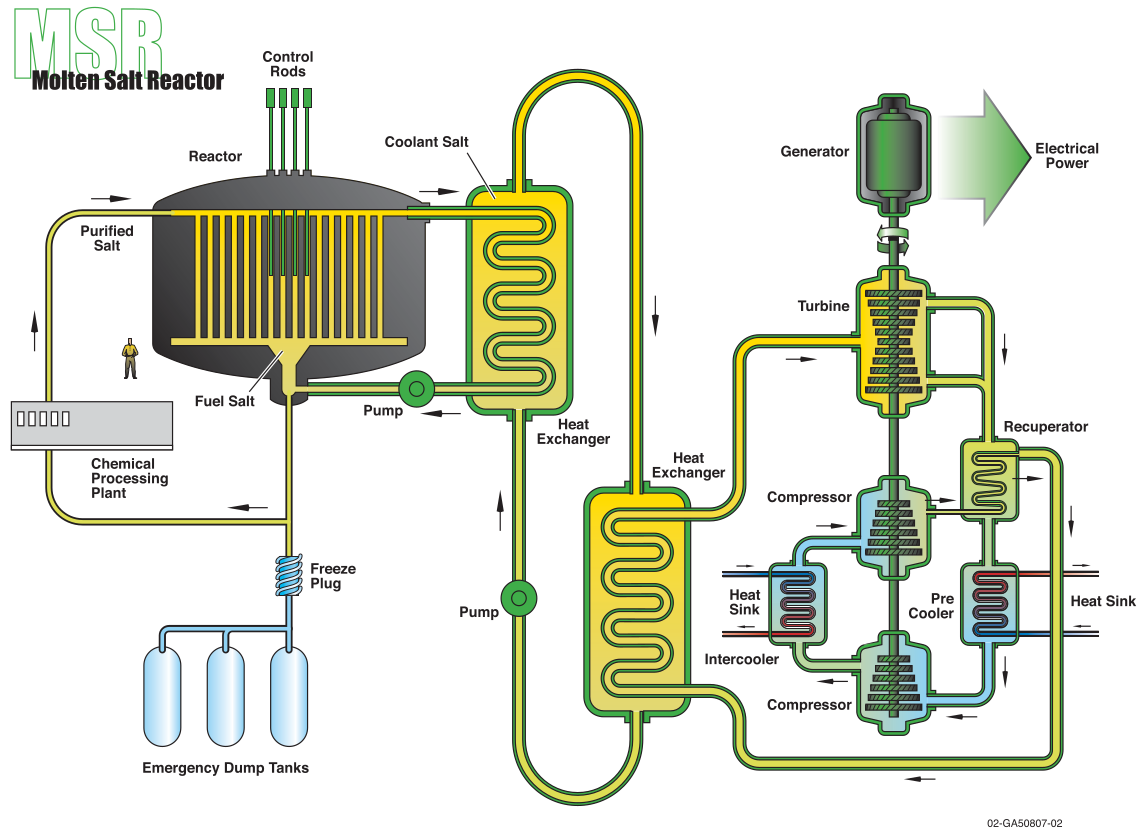
\includegraphics[width=.5\textwidth]{./images/msr}
			\caption{Schematic diagram of a general \gls{MSR} concept.}
			\label{fig:msr}
		\end{figure}
\end{frame}

\begin{frame}
	\frametitle{Molten Salt Reactors}
		\textbf{Characteristics and challenges}
		\begin{itemize}
			\item Strong coupling between neutronics and thermal-hydraulics
			\begin{itemize}
				\item Strong Doppler and density feedback in the fuel salt
				\item Relatively more prompt response expected compared to
				existing LWRs
			\end{itemize}
			\item Movement and decay of delayed neutron precursors in the molten
			salt loop
			\begin{itemize}
				\item Conventional safety analysis codes do not account for the
				delayed neutron precursor movement
			\end{itemize}
			\item Constantly evolving fuel composition across the lifetime of an
			\gls{MSR}
			\begin{itemize}
				\item Reactor safety parameters and transient response may be
				different for \gls{BOL} vs \gls{EOL} fuel compositions
			\end{itemize}
		\end{itemize}
\end{frame}

\subsection{Moltres}
\begin{frame}
	\frametitle{Moltres}
		\textbf{What is Moltres?}
		\begin{itemize}
			\item Moltres \cite{lindsay_introduction_2018} is an application
			built on the \gls{MOOSE} framework, for the simulation of \glspl{MSR}
			\item \gls{MOOSE} \cite{gaston_moose:_2009} is an open source finite
			element framework written in \texttt{C++} that
			relies on Libmesh and PETSc for advanced meshing and PDE solving
			capabilities
			\item Moltres can run transient, implicitly coupled
			neutronics/thermal-hydraulics simulations
			\begin{itemize}
				\item Multi-group neutron diffusion (arbitrary no. of groups)
				\item \gls{DNP} decay (with advection)
				\item Incompressible Navier-Stokes for temperature
				advection-diffusion
				\item 1D, 2D, and 3D modeling are supported
			\end{itemize}
		\end{itemize}
\end{frame}
\subsection{Objectives}
\begin{frame}
	\frametitle{Objectives}
		\textbf{Objectives}
		\begin{itemize}
			\item Verify the neutronics capabilities in Moltres against Serpent
			\item Demonstrate coupled neutronics/thermal-hydraulics simulations
			of the \gls{MSFR} concept,
			\begin{itemize}
				\item with \gls{BOL}, early-life, and \gls{EOL} fuel compositions
				\item for steady state and transient cases: \gls{ULOHS} accident
			\end{itemize}
		\end{itemize}
\end{frame}

\section{Method}
\subsection{Molten Salt Fast Reactor}
\begin{frame}
	\frametitle{Molten Salt Fast Reactor}
		\textbf{Features}
		\begin{itemize}
			\item Fast-spectrum \gls{MSR} concept
			\item Can run on the open U/Pu, U/TRU or closed U/Th fuel cycles
			\item Primary fuel salt flows upwards through the central core
			region and separates into 16 smaller external loops towards the
			heat exchangers and pumps
			\item Radially surrounded by a tank of blanket salt consisting of
			fertile isotopes such as $^{232}$Th for breeding
		\end{itemize}
		\begin{columns}
			\column[t]{3.5cm}
			\begin{figure}
				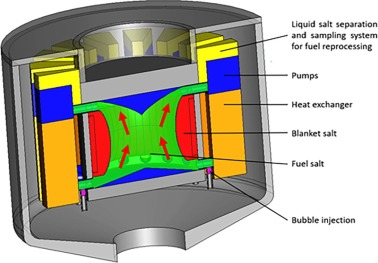
\includegraphics[width=\textwidth]{../paper/figures/MSFR}
				\caption{\gls{MSFR} concept}
			\end{figure}
			\column[t]{6.5cm}
			{\footnotesize
			\begin{table}[h]
				\caption{\footnotesize Specifications of the \gls{MSFR} design
				\cite{serp_molten_2014}.}
				\begin{tabular}{ l l }
				\hline
				Parameter & Value \\
				\hline
				Thermal/Electric output [MW$_{\text{th}}$/MW$_{\text{e}}$] &
				3000 / 1500 \\
				Salt volume [m$^3$] & 18 \\
				Salt fraction in core & 0.5 \\
				Number of circulation loops & 16 \\
				Nominal flow rate [kg s$^{-1}$] & 18500  \\
				Nominal circulation time [s] & 4.0 \\
				Inlet/outlet temperature [K] & 923 / 1023 \\
				Blanket volume [m$^3$] & 7.3\\
				\hline
				\end{tabular}
			\label{table:msfr}
			\end{table}
			}
		\end{columns}
\end{frame}
\subsection{Moltres}
\begin{frame}
	\frametitle{Moltres}
	\begin{columns}
		\column{5cm}
		Moltres solves the implicitly coupled governing equations for
		neutron diffusion, \gls{DNP} concentrations, and
		temperature.
		
		\vspace{.2cm}
		Moltres requires neutron group constant data, available from any neutron
		transport code (e.g. Serpent, SCALE), for the neutronics calculations.
		
		\vspace{.2cm}
		Moltres accepts various mesh file formats (e.g. exodus, gmsh, etc.)
		\column{5cm}
		\begin{figure}
			\centering
			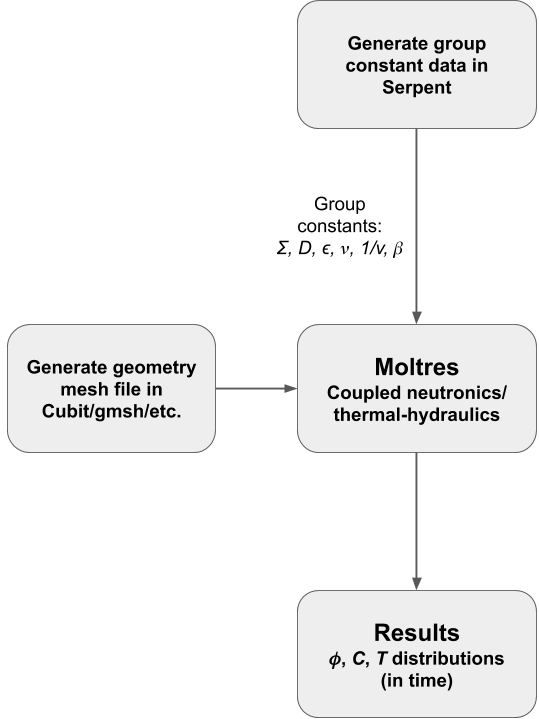
\includegraphics[width=.9\textwidth]{./images/flowchart}
			\caption{Flowchart for running a Moltres simulation.}
			\label{fig:flowchart}
		\end{figure}
	\end{columns}
\end{frame}

\begin{frame}
	\frametitle{Moltres}
	\textbf{Multi-group neutron diffusion}
		\begin{align}
	\frac{1}{v_g} &\frac{\partial \phi_g}{\partial t} - \nabla \cdot D_g \nabla
	\phi_g + \Sigma^r_g \phi_g \nonumber \\ 
	&= \sum^G_{g \neq g'} \Sigma^s_{g' \rightarrow g} \phi_{g'} + \chi^p_g
	\sum^G_{g'=1} (1-\beta) \nu \Sigma^f_{g'} \phi_{g'} + \chi^d_g \sum^I_i
	\lambda_i C_i \label{eq1}
		\end{align}
	\textbf{\gls{DNP} concentration (with advection)}
		\begin{align}
	\frac{\partial C_i}{\partial t} = \sum^G_{g'=1} \beta_i \nu \Sigma^f_{g'}
	\phi_{g'} - \lambda_i C_i
	{\color{red}
	 - \nabla \cdot \overrightarrow{u} C_i}
	\label{eq2}
		\end{align}
		
		Additional advection term in the \gls{DNP} concentration
		equations to account for fuel advection effects.
\end{frame}

\begin{frame}
	\frametitle{Moltres}
		\textbf{Temperature advection-diffusion}
		\begin{align}
	\rho c_{p} \frac{\partial T}{\partial t} + \nabla \cdot \big( \rho
	c_{p} \overrightarrow{u} T - k \nabla T \big) = Q_s - Q_{hx}
	\label{eq3}
		\end{align}
		
		where
		\begin{align*}
		Q_s = \sum^G_{g=1} \epsilon_g \Sigma_g^f \phi_g \label{eq4}
		\end{align*}
		
		Moltres has access to the Navier-Stokes module on \gls{MOOSE} for
		simulating flow. For this work, we assumed plug flow (uniform flow).
\end{frame}

%\begin{frame}
%	\frametitle{Moltres}
%	\textbf{\gls{DNP} drift and decay}
%		\begin{itemize}
%			\item A significant fraction of \gls{DNP} decay outside the active
%			core region
%			\item Moltres 
%		\end{itemize}
%\end{frame}

%\subsection{Study Approach}
%\begin{frame}
	\frametitle{Study Approach}
		\textbf{1) Neutronics verification} \\
		\begin{itemize}
			\item Obtain \gls{MSFR} \gls{BOL}, early-life, and \gls{EOL} fuel
			compositions under the U/Th breeder configuration (available from
			Rykhlevskii et al. \cite{rykhlevskii_fuel_2019})
			\item Perform neutronics calculations on the Serpent 2 Monte Carlo
			transport code and generate
		\end{itemize}
\end{frame}

\section{Results}
%\input{breakdown}
%\subsection{Comparison of Prediction Methods}
%\input{compare_prediction}
%\subsection{Sensitivity Analysis of Power Buffer Size}
%\input{sa}
%\subsection{Best Performing Transition Scenarios}
%\input{best}

\section{Conclusion}
\subsection{Conclusion}
%\begin{frame}
	\frametitle{Conclusion}
		The neutron group fluxes and reactivity coefficients from Moltres
		(without \gls{DNP} drift) are in
		good agreement with Serpent results, in the context of the \gls{MSFR}.
		
		\vspace{.3cm}
		The steady state neutron flux, temperature, and \gls{DNP} distributions
		observed are expected for uniform flow.
		
		\vspace{.3cm}
		Discrepancies in peak neutron
		flux and temperature distributions to other work are primarily due to
		the minor differences in core geometry and using uniform flow instead of
		appling a turbulence model.
		
		\vspace{.3cm}
		Higher core temperatures observed for start-up fuel composition than
		early-life and equilibrium compositions.
		
		\vspace{.3cm}
		Discrepancy in average core temperatures during \gls{ULOHS} is mainly due
		to the lack of a decay heat model in Moltres.
\end{frame}
\subsection{Future Work}
%\input{future_work}
%\begin{frame}
	\frametitle{Acknowledgments}
    	Sun Myung Park is supported by the Singapore Nuclear Research and Safety
    	Initiative (SNRSI) Postgraduate Scholarship.
    	
    	\vspace{.3cm}
    	Andrei Rykhlevskii and Dr Kathryn Huff are both supported by funding from
    	the DOE ARPA-E MEITNER Program (award DE-AR0000983).
    	
    	\vspace{.3cm}
    	Dr Kathryn Huff is also supported by the Blue Waters sustained-petascale
    	computing project supported by the National Science Foundation.
\end{frame}

\begin{frame}
	\large
	\centering
	\textbf{Thank you for your attention!}
\end{frame}

%%--------------------------------%%
%%--------------------------------%%
\begin{frame}[allowframebreaks]
  \frametitle{References}
  \bibliographystyle{plain}
  {\footnotesize \bibliography{./bibliography.bib} }

\end{frame}

%%--------------------------------%%


\end{document}

